\section{222 --- Count Complete Tree Nodes}

\textbf{Medium}

Given a complete binary tree, count the number of nodes.

\paragraph{Note:}

Definition of a complete binary tree from \textbf{Wikipedia}:

In a complete binary tree every level, except possibly the last, is completely filled, and all nodes in the last level are as far left as possible. It can have between 1 and $2^h$ nodes inclusive at the last level $h$.

\paragraph{Example:}
\begin{flushleft}


\textbf{Input}: 

\begin{figure}[H]
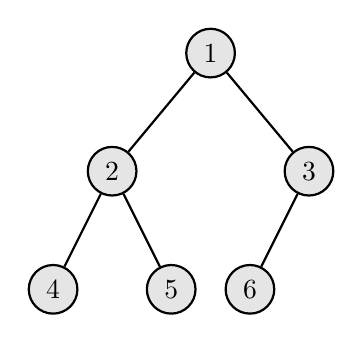
\begin{tikzpicture}
[every node/.style={draw, circle, fill=gray!20!, minimum size=5mm},
level 1/.style={sibling distance=25mm},
level 2/.style={sibling distance=15mm},
thick]
\node{1}
child{node{2} child{node{4}} child{node{5}}}
child{node{3} child{node{6}} child[missing]};
\end{tikzpicture}
\end{figure}

\textbf{Output}: 6
\end{flushleft}

\subsection{Binary Search}
In a complete binary tree every level, except possibly the last, is completely filled, and all nodes in the last level are as far left as possible.

Suppose the level of the tree is $d$ (level is from 0 to $d$). The number of nodes in all levels but the last one is $2^d - 1$. The number of nodes in the last level could vary from 1 to $2^d$.

Enumerate potential nodes from 0 to $2^d - 1$1 and perform the binary search by the node index to check how many nodes are in the last level.

\setcounter{lstlisting}{0}
\begin{lstlisting}[style=customc, caption={Binary Search}]
int countNodes( TreeNode* root )
{

    if( !root )
    {
        return 0;
    }
    //get the depth of tree
    //tree are from level 0 to level d
    auto d( get_depth( root ) );
    if( d == 0 )
    {
        return 1;
    }
    //find if a index in the last level exists
    int left = 0;
    int right = ( 1 << d ) - 1;
    while( left <= right )
    {
        auto mid( left + ( right - left ) / 2 );
        if( found( mid, d, root ) )
        {
            left = mid + 1;
        }
        else
        {
            right = mid - 1;
        }
    }
    //level 0 to level (d-1) we have 2^d-1 nodes
    //and (left) nodes at level (d)
    return ( 1 << d ) - 1 + left;
}
//helper function to get depth
int get_depth( TreeNode* node )
{
    int d = 0;
    while( node->left )
    {
        ++d;
        node = node->left;
    }
    return d;
}
//helper function to check if a node with (idx)
//exists at level d
bool found( int idx, int d, TreeNode* node )
{
    //at level d
    //index of each node is from 0
    //to (2^d-1) for complete binary tree
    int left = 0;
    int right = ( 1 << d ) - 1;
    for( int level = 0; level < d; ++level )
    {
        auto mid( left + ( right - left ) / 2 );
        if( idx <= mid )
        {
            //idx in left child tree
            //search range is [left, mid]
            right = mid;
            node = node->left;
        }
        else
        {
            //idx in right child tree
            //search range is [mid+1,right]
            left = mid + 1;
            node = node->right;
        }
    }
    return node;
}
\end{lstlisting}

\subsection{Iterative Approach}
We can find the leftmost and rightmost path from \fcj{root} to the leaf node. If the lengths of both are equal, the last level will have $2^d-1$ nodes (perfect binary tree). Otherwise, the number of nodes in the left and right subtree is the answer.

\begin{lstlisting}[style=customc, caption={Recursive}]
int countNodes( TreeNode* root )
{
    auto ltree = root;
    auto d_left( 0 );
    while( ltree )
    {
        ltree = ltree->left;
        ++d_left;
    }
    auto rtree = root;
    auto d_right( 0 );
    while( rtree )
    {
        rtree = rtree->right;
        ++d_right;
    }
    if( d_left == d_right )
    {
        //perfert complete binary tree
        return ( 1 << d_left ) - 1;
    }
    //otherwise return the left and right subtree nodes
    return countNodes( root->left ) + countNodes( root->right ) + 1;
}
\end{lstlisting}